\documentclass[12pt,a4paper]{article}

\usepackage[a4paper,margin=1in]{geometry}
\usepackage{graphicx}
\usepackage{booktabs}
\usepackage{amsmath,amssymb}
\usepackage{float}
\usepackage{hyperref}
\usepackage{xcolor}
\usepackage{listings}
\usepackage{enumitem}
\usepackage{fancyhdr}
\usepackage{longtable}

\hypersetup{colorlinks=true,linkcolor=blue,urlcolor=blue,citecolor=blue}

\pagestyle{fancy}
\setlength{\headheight}{14.5pt}
\fancyhf{}
\lhead{ICS1512}
\rhead{Machine Learning Algorithms Laboratory}
\cfoot{\thepage}

\lstset{
language=Python,
basicstyle=\ttfamily\small,
numbers=left,
frame=single,
breaklines=true,
showstringspaces=false
}

\setlength{\parskip}{4pt}

\begin{document}

\begin{tabular}{|p{4cm}|p{10.5cm}|}
\hline
Experiment No. & 8 \\ \hline
Experiment Title &
Clustering Human Activity Recognition Data using K-Means, DBSCAN and Hierarchical Clustering\footnotemark \\ \hline
Student Name & Sundareswaran R \\ \hline
Register Number & 3122247001048 \\ \hline
Faculty & Dr. Poreddy Ajay Kumar Reddy \\ \hline
Submission Date & \today \\ \hline
\end{tabular}
\footnotetext{\textbf{GitHub Repository: }\url{https://github.com/The-FOOL-00/ML_Lab}}

% ------------------------------------------------------------------
\section{Objective}
To cluster the UCI Human Activity Recognition (HAR) smartphone data with K-Means, DBSCAN and Hierarchical Agglomerative Clustering (HAC), to select the parameters of each method (number of clusters $k$, $\epsilon$, minPts, linkage), and to compare the clusters with the true activity labels using internal and external clustering metrics.

% ------------------------------------------------------------------
\section{Problem Statement}
\textbf{Input:} 10,299 windows of smartphone accelerometer and gyroscope signals, each described by 561 time- and frequency-domain features.\\
\textbf{Output:} a cluster label for every window, found without using the activity labels.\\
\textbf{Objective:} group the windows so that they match the physical activities, decide the number of clusters (K-Means, HAC) and the density parameters (DBSCAN), and measure how closely each clustering agrees with the six real activities.

% ------------------------------------------------------------------
\section{Dataset Description}
\begin{longtable}{|p{4.6cm}|p{10cm}|}
\hline
Dataset Name & Human Activity Recognition Using Smartphones (UCI HAR) \\ \hline
Dataset Source & UCI Machine Learning Repository, ID 240 \cite{anguita2013,uci_har}, \url{https://archive.ics.uci.edu/dataset/240} \\ \hline
Number of Samples & 10,299 windows (7,352 train + 2,947 test files) from 30 volunteers \\ \hline
Number of Features & 561 numeric features (\texttt{subject} and \texttt{Activity} are not used for clustering) \\ \hline
Number of Classes & 6 activities, used only for evaluation \\ \hline
Missing Values & 0 \\ \hline
Train-Test Split & Not used (unsupervised); the train and test files are merged \\ \hline
\end{longtable}

The six activities are WALKING, WALKING\_UPSTAIRS, WALKING\_DOWNSTAIRS, SITTING, STANDING and LAYING. The signals were recorded at 50 Hz with the accelerometer and gyroscope of a waist-mounted smartphone (volunteers aged 19--48), cut into windows of 2.56 s (128 readings) and converted into 561 time- and frequency-domain features.

% ------------------------------------------------------------------
\section{Exploratory Data Analysis}\label{sec:eda}
The EDA function of the notebook was run on the merged table (features + \texttt{subject} + \texttt{Activity}). Its main results are given below.

\textbf{Dataset overview and missing value analysis.}

\begin{center}
\small
\begin{tabular}{ll}
\toprule
Item & Value \\
\midrule
Shape (rows $\times$ columns) & $10299 \times 563$ \\
Feature columns & 561 (\texttt{float64}), all values lie in $[-1,1]$ \\
\texttt{subject} & \texttt{int64}, volunteer id 1--30 \\
\texttt{Activity} (target) & \texttt{object}, 6 categories \\
Missing values & 0 in all 563 columns (0.0\%) \\
Duplicate rows & 0 \\
\bottomrule
\end{tabular}
\end{center}

\textbf{Statistical summary.} The EDA function ranks the numeric features by ANOVA F-score against the activity and keeps the top 10 for plotting. The first five are summarised below.

\begin{center}
\small
\begin{tabular}{lrrrr}
\toprule
Feature & Mean & Std & Min & Max \\
\midrule
fBodyAccJerk-entropy()-X & $-0.267$ & 0.749 & $-1$ & 1 \\
tGravityAcc-mean()-X & 0.669 & 0.515 & $-1$ & 1 \\
tGravityAcc-min()-X & 0.684 & 0.507 & $-1$ & 1 \\
tGravityAcc-max()-X & 0.609 & 0.509 & $-1$ & 1 \\
tGravityAcc-energy()-X & 0.446 & 0.696 & $-1$ & 1 \\
\bottomrule
\end{tabular}
\end{center}

\subsection*{Class Distribution}

\begin{figure}[H]
\centering
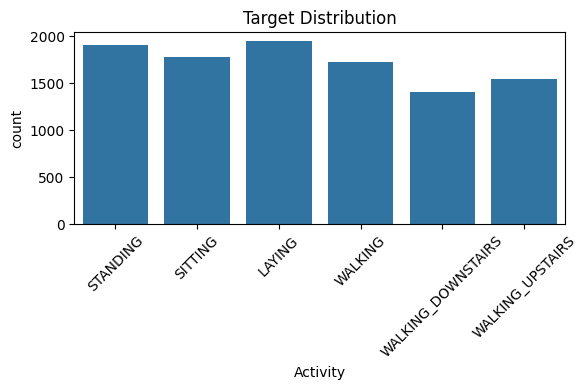
\includegraphics[width=0.48\linewidth]{figures/fig_class_distribution.png}
\caption{Number of windows per activity.}
\label{fig:class}
\par\medskip
\begin{minipage}{\linewidth}
\raggedright\setlength{\parskip}{0pt}
\textbf{Inference:} LAYING is the largest class (1,944 windows) and WALKING\_DOWNSTAIRS the smallest (1,406). The ratio between them is only about 1.4, so the data is nearly balanced and no resampling is needed. Because the classes have similar sizes, a poor agreement between clusters and activities cannot be blamed on class imbalance. The labels are used only to evaluate the clusters, never to build them.
\end{minipage}
\end{figure}

\subsection*{Feature Distribution}

\begin{figure}[H]
\centering
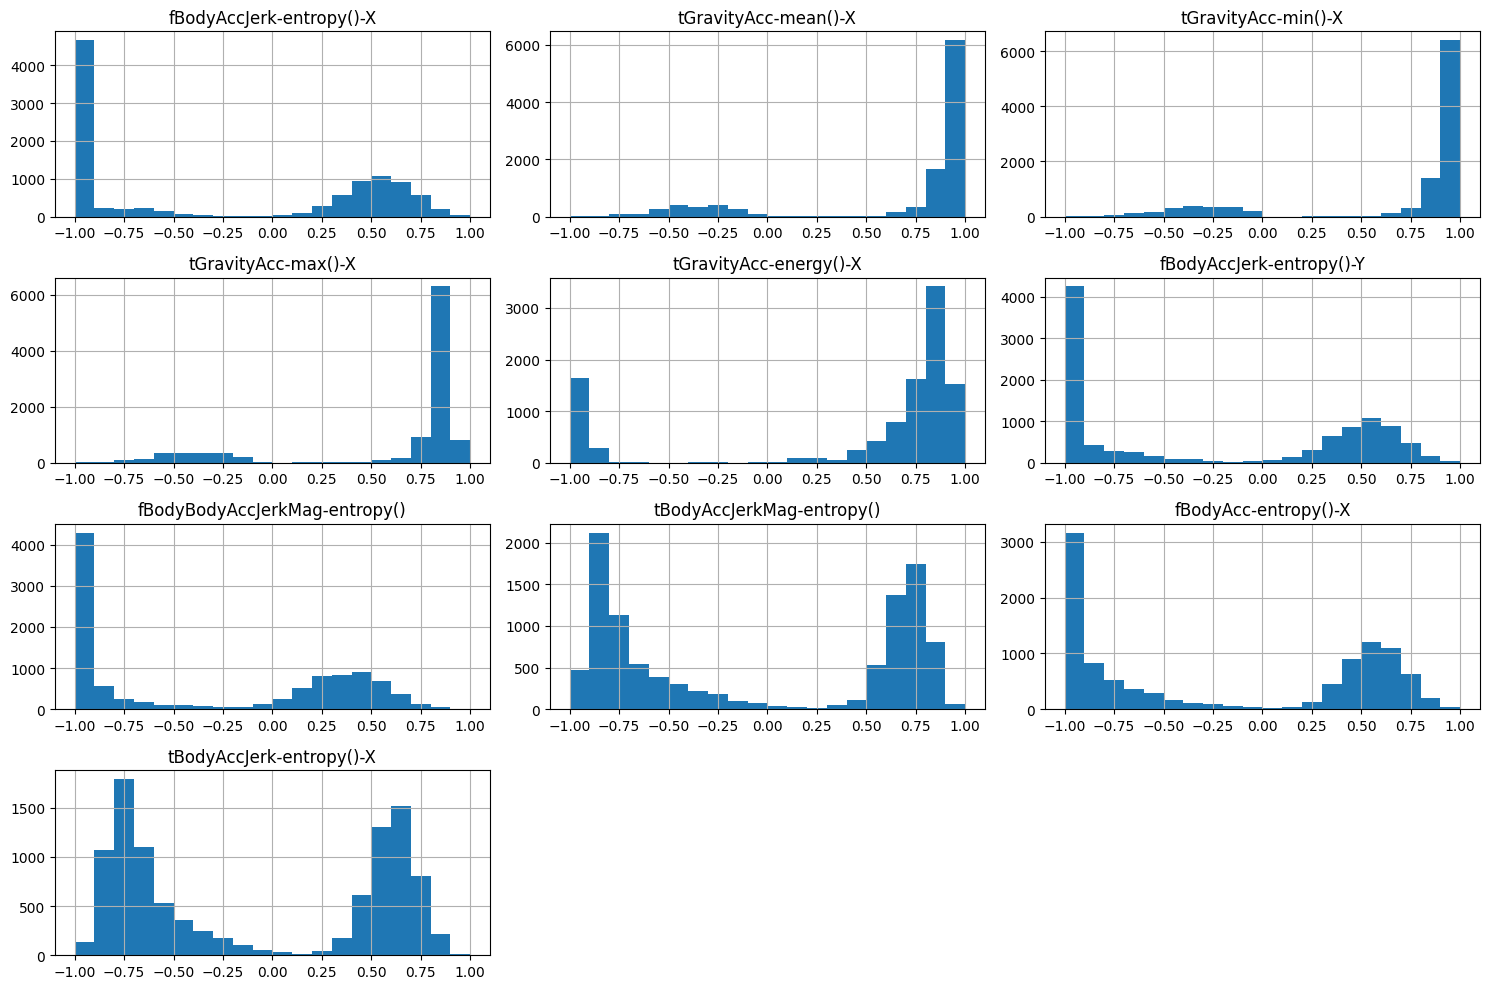
\includegraphics[width=0.82\linewidth]{figures/fig_feature_histograms.png}
\caption{Histograms of the 10 features with the highest F-score.}
\label{fig:hist}
\par\medskip
\begin{minipage}{\linewidth}
\raggedright\setlength{\parskip}{0pt}
\textbf{Inference:} Most of the selected features have two separate peaks. The entropy features have a large spike at $-1$ (static activities) and a second hump between 0.25 and 0.75 (walking activities). The gravity features are concentrated near $+1$ with a smaller group between $-0.75$ and $-0.1$, which corresponds to the LAYING posture. This two-peak shape suggests that the data contains two broad groups, static and dynamic, and that all features are already bounded in $[-1,1]$.
\end{minipage}
\end{figure}

\subsection*{Correlation Matrix}

\begin{figure}[H]
\centering
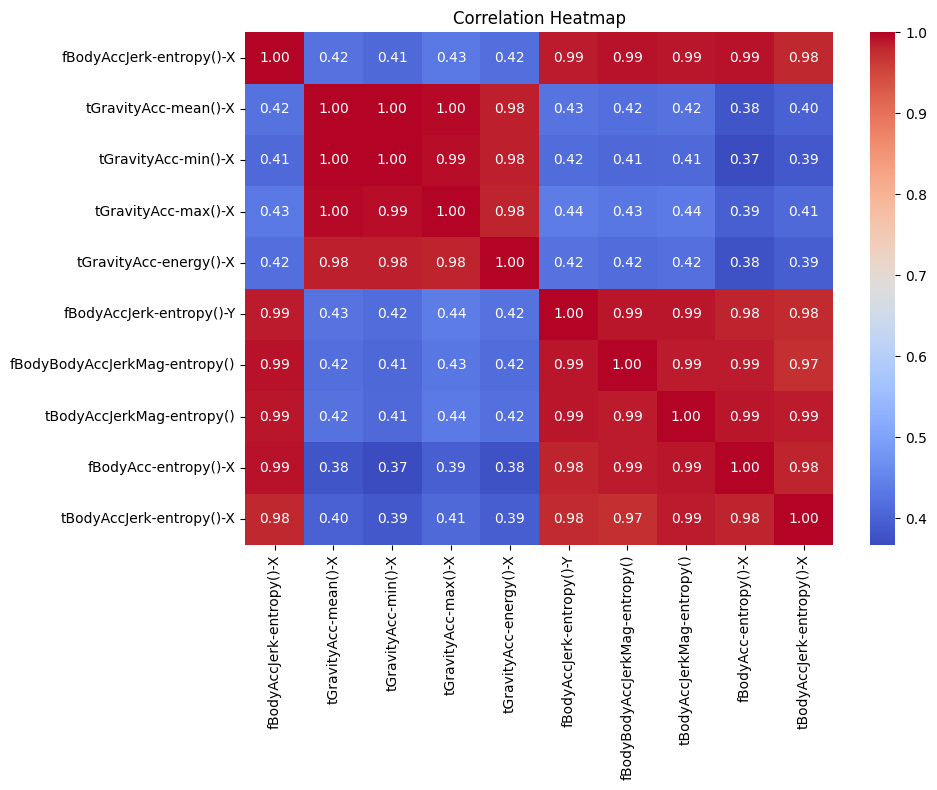
\includegraphics[width=0.6\linewidth]{figures/fig_correlation_heatmap.png}
\caption{Correlation matrix of the 10 selected features.}
\label{fig:corr}
\par\medskip
\begin{minipage}{\linewidth}
\raggedright\setlength{\parskip}{0pt}
\textbf{Inference:} The features form two blocks. Inside the entropy block the correlation is 0.97--0.99, and inside the gravity block it is 0.98--1.00, while the correlation between the blocks is only 0.37--0.44. So the features are highly redundant, and they carry two different kinds of information: motion intensity and body orientation. This redundancy is the reason for applying PCA before clustering.
\end{minipage}
\end{figure}

\subsection*{Relationship between Features and Activities}

\begin{figure}[H]
\centering
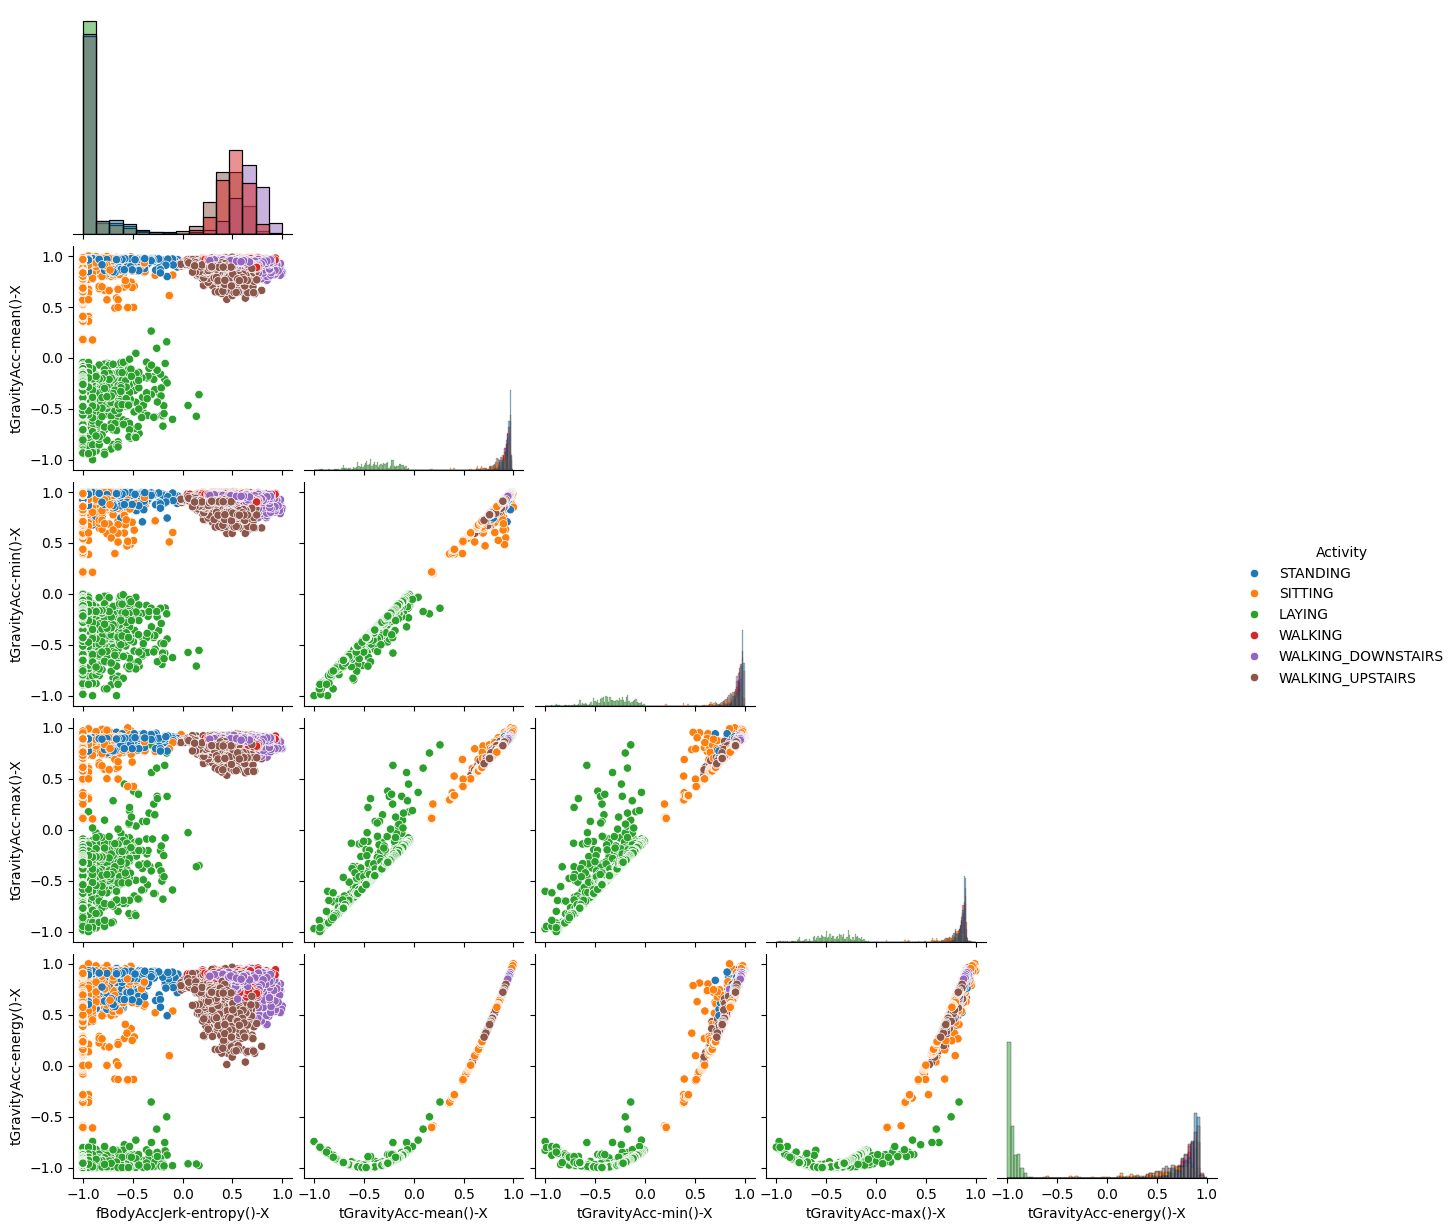
\includegraphics[width=0.68\linewidth]{figures/fig_pairplot.png}
\caption{Pair plot of the top five features, coloured by activity.}
\label{fig:pair}
\par\medskip
\begin{minipage}{\linewidth}
\raggedright\setlength{\parskip}{0pt}
\textbf{Inference:} LAYING (green) is clearly separated from the other activities on the tGravityAcc features. The entropy feature separates the three walking activities (positive values) from the three static ones (close to $-1$). SITTING and STANDING overlap almost completely in every panel, and the three walking activities also overlap each other, with WALKING\_UPSTAIRS shifted slightly towards lower gravity values. It can therefore be expected that clustering will find static versus dynamic and LAYING easily, but not sitting versus standing.
\end{minipage}
\end{figure}

% ------------------------------------------------------------------
\section{Data Preprocessing}
\begin{itemize}
\item \textbf{Missing value handling:} no missing values were found. The notebook still fills numeric gaps with the column median as a safeguard.
\item \textbf{Encoding:} the activity ids of the label files are mapped to activity names with the file \texttt{activity\_labels.txt} and then label-encoded (LAYING = 0, SITTING = 1, STANDING = 2, WALKING = 3, WALKING\_DOWNSTAIRS = 4, WALKING\_UPSTAIRS = 5). The codes are used only for evaluation.
\item \textbf{Feature scaling:} \texttt{StandardScaler} converts every feature to zero mean and unit variance, $z=(x-\mu)/\sigma$, because clustering depends on distances.
\item \textbf{Train-test split:} none, since clustering is unsupervised. The train and test files are concatenated.
\item \textbf{Feature engineering:} \texttt{subject} and \texttt{Activity} are removed from the feature matrix. PCA \cite{jolliffe2016} on the scaled data keeps the first 104 components, which explain 95.05\% of the variance (561 $\rightarrow$ 104 features). These components are the input of all three algorithms, and the first two components are used only for the 2-D plots.
\end{itemize}

% ------------------------------------------------------------------
\section{Machine Learning Algorithm}

\subsection*{Model A: K-Means}
\textbf{Working principle.} K-Means \cite{lloyd1982} initialises $k$ centroids (k-means++), every point is assigned to its nearest centroid, each centroid is moved to the mean of its points, and the last two steps are repeated until the assignments stop changing.

\textbf{Mathematical formulation.} K-Means minimises the within-cluster sum of squares (WCSS, the inertia)
\begin{equation}
J=\sum_{j=1}^{k}\sum_{\mathbf{x}_i\in C_j}\lVert \mathbf{x}_i-\boldsymbol{\mu}_j\rVert^{2}, \qquad \boldsymbol{\mu}_j=\frac{1}{|C_j|}\sum_{\mathbf{x}_i\in C_j}\mathbf{x}_i .
\end{equation}

\textbf{Advantages:} simple, fast, and works well for compact, roughly spherical clusters. \textbf{Limitations:} $k$ must be given, the result depends on the initialisation, it is sensitive to outliers, and it cannot find clusters of arbitrary shape.

\subsection*{Model B: DBSCAN}
\textbf{Working principle.} DBSCAN \cite{ester1996}: a point is a \emph{core point} if at least minPts points (including itself) lie within distance $\epsilon$. Core points that are within $\epsilon$ of each other are joined into one cluster, points inside the $\epsilon$-neighbourhood of a core point but not core themselves are \emph{border points}, and all remaining points are \emph{noise} (label $-1$).

\textbf{Mathematical formulation.}
\begin{equation}
N_\epsilon(p)=\{q\in D:\ d(p,q)\le\epsilon\},\qquad p\ \text{is core}\iff |N_\epsilon(p)|\ge \text{minPts}.
\end{equation}

\textbf{Advantages:} $k$ is not needed, clusters can have any shape, and noise is detected. \textbf{Limitations:} the result is very sensitive to $\epsilon$ and minPts, one $\epsilon$ cannot handle clusters of different density, and distances lose contrast in high-dimensional data.

\subsection*{Model C: Hierarchical Agglomerative Clustering (Ward)}
\textbf{Working principle.} Every point starts as its own cluster and the two ``closest'' clusters are merged repeatedly until one cluster is left. The merge history is drawn as a dendrogram, and cutting it at a chosen height gives $k$ clusters.

\textbf{Mathematical formulation.} Ward's linkage \cite{ward1963} merges the pair $(A,B)$ that gives the smallest increase in the within-cluster variance
\begin{equation}
\Delta(A,B)=\frac{|A|\,|B|}{|A|+|B|}\,\lVert \boldsymbol{\mu}_A-\boldsymbol{\mu}_B\rVert^{2}.
\end{equation}
The other linkages differ in the cluster distance: single = minimum, complete = maximum, average = mean pairwise distance.

\textbf{Advantages:} $k$ can be chosen after looking at the dendrogram, and Ward gives compact clusters of similar size. \textbf{Limitations:} it needs $O(n^2)$ memory and time, merges cannot be undone, and single linkage suffers from chaining.

\subsection*{Evaluation metrics}
Internal metrics (no labels): the silhouette $s(i)=\dfrac{b(i)-a(i)}{\max\{a(i),b(i)\}}$ where $a$ is the mean distance to the own cluster and $b$ the mean distance to the nearest other cluster (higher is better); the Davies--Bouldin index $\frac{1}{k}\sum_i\max_{j\ne i}\frac{s_i+s_j}{d_{ij}}$ (lower is better); and the Calinski--Harabasz index $\dfrac{\operatorname{tr}(B_k)/(k-1)}{\operatorname{tr}(W_k)/(n-k)}$ (higher is better) \cite{rousseeuw1987,davies1979,calinski1974}. External metrics (with the true activities): the Adjusted Rand Index (ARI), which is the Rand index corrected for chance \cite{hubert1985}, and the Normalized Mutual Information $\mathrm{NMI}=\dfrac{2\,I(U;V)}{H(U)+H(V)}$ \cite{strehl2002}.

% ------------------------------------------------------------------
\section{Experimental Setup}
\begin{tabular}{lp{11cm}}
\toprule
Python Version & 3.12.3 \\
Scikit-Learn Version & 1.8.0 \cite{pedregosa2011} (with pandas 3.0.2, NumPy 2.4.4, SciPy 1.17.1, Matplotlib 3.10.8, Seaborn 0.13.2) \\
IDE & Jupyter Notebook (ipykernel 7.3.0) \\
Operating System & Ubuntu 24.04.4 LTS \\
Hardware & Intel Xeon @ 2.10 GHz, 1 vCPU, about 4 GB RAM \\
\bottomrule
\end{tabular}

% ------------------------------------------------------------------
\section{Hyperparameter Selection}\label{sec:hyper}

\begin{tabular}{lp{10.5cm}}
\toprule
Parameter & Value\\
\midrule
PCA components & 104 (smallest number reaching 95\% variance) \\
K-Means: $k$ & searched for $k=2,\dots,8$; best $k=2$ (highest silhouette); $k=6$ (number of activities) also evaluated \\
K-Means: other & \texttt{n\_init}=10, \texttt{random\_state}=42, Euclidean distance \\
DBSCAN: $\epsilon$ & 12.90, taken from the 70th percentile of the 5-th neighbour distances (k-distance graph) \\
DBSCAN: minPts & 5 (5, 10 and 20 were tried) \\
HAC: linkage & Ward (single, complete and average compared) \\
HAC: $k$ & 2 and 6 (same as K-Means) \\
\bottomrule
\end{tabular}

\subsection*{K-Means: elbow method (Table 1 of the assignment)}
\begin{center}
\small
\begin{tabular}{ccc}
\toprule
Number of clusters $k$ & WCSS (inertia) & Silhouette score \\
\midrule
2 & 2,986,709 & \textbf{0.413} \\
3 & 2,635,081 & 0.331 \\
4 & 2,495,681 & 0.162 \\
5 & 2,369,136 & 0.140 \\
6 & 2,291,589 & 0.122 \\
7 & 2,234,409 & 0.089 \\
8 & 2,180,422 & 0.083 \\
\bottomrule
\end{tabular}
\end{center}

\subsection*{DBSCAN: parameter grid}
$\epsilon$ was taken from the 70th, 80th, 90th and 95th percentile of the k-distances for each minPts. A setting was accepted if it had at least 2 clusters, at most 30\% noise and no cluster holding more than 60\% of the points (a setting with 97\% of the points in one cluster can have a good silhouette but separates nothing). The accepted setting with the best silhouette was selected (first row, in bold).

\begin{center}
\small
\begin{tabular}{rrrrrr}
\toprule
$\epsilon$ & minPts & Clusters & Noise \% & Largest cluster \% & Silhouette \\
\midrule
\textbf{12.90} & \textbf{5} & \textbf{19} & \textbf{22.6} & \textbf{51.0} & \textbf{0.305} \\
14.24 & 5 & 18 & 13.7 & 84.5 & 0.140 \\
16.20 & 5 & 6 & 6.4 & 92.9 & 0.056 \\
18.45 & 5 & 4 & 3.2 & 96.7 & 0.342 \\
13.80 & 10 & 11 & 20.0 & 51.8 & 0.303 \\
15.26 & 10 & 3 & 11.1 & 88.5 & 0.320 \\
17.31 & 10 & 2 & 5.4 & 94.2 & 0.333 \\
19.84 & 10 & 1 & 2.6 & 97.4 & -- \\
14.64 & 20 & 3 & 18.6 & 80.9 & 0.303 \\
16.21 & 20 & 2 & 9.4 & 90.3 & 0.342 \\
18.39 & 20 & 1 & 4.8 & 95.2 & -- \\
21.12 & 20 & 1 & 2.1 & 97.9 & -- \\
\bottomrule
\end{tabular}
\end{center}

% ------------------------------------------------------------------
\section{Results}
\begin{samepage}
Accuracy, precision, recall, F1-score and ROC-AUC need predicted class labels or scores from a trained classifier, so they are not defined for unsupervised clustering. The corresponding measures for clustering are given instead: three internal metrics and two external metrics (computed against the true activities). The best value in each row is in bold. For DBSCAN the internal metrics ignore the noise points, and ARI/NMI treat noise as one extra group.

\begin{center}
\small
\setlength{\tabcolsep}{3pt}
\begin{tabular}{lccccc}
\toprule
Metric & \begin{tabular}[c]{@{}c@{}}K-Means\\($k=2$)\end{tabular} & \begin{tabular}[c]{@{}c@{}}K-Means\\($k=6$)\end{tabular} & DBSCAN & \begin{tabular}[c]{@{}c@{}}HAC-Ward\\($k=2$)\end{tabular} & \begin{tabular}[c]{@{}c@{}}HAC-Ward\\($k=6$)\end{tabular} \\
\midrule
Clusters & 2 & 6 & 19 (+ noise) & 2 & 6 \\
Silhouette $\uparrow$ & \textbf{0.413} & 0.122 & 0.305 & 0.412 & 0.117 \\
Davies--Bouldin $\downarrow$ & \textbf{1.019} & 2.239 & 1.448 & 1.020 & 2.248 \\
Calinski--Harabasz $\uparrow$ & \textbf{8635.8} & 2874.6 & 463.0 & 8611.8 & 2660.7 \\
ARI $\uparrow$ & 0.330 & 0.419 & 0.311 & 0.333 & \textbf{0.500} \\
NMI $\uparrow$ & 0.545 & 0.559 & 0.456 & 0.557 & \textbf{0.624} \\
\bottomrule
\end{tabular}
\end{center}
\end{samepage}

\textbf{Effect of the linkage} (HAC with 6 clusters on the same data):
\begin{center}
\small
\begin{tabular}{lcccc}
\toprule
Linkage & Silhouette & ARI & NMI & Largest cluster \% \\
\midrule
Single & 0.557 & 0.000 & 0.001 & 99.94 \\
Complete & 0.321 & 0.006 & 0.045 & 95.29 \\
Average & 0.442 & 0.000 & 0.005 & 99.76 \\
Ward & 0.117 & \textbf{0.500} & \textbf{0.624} & 34.15 \\
\bottomrule
\end{tabular}
\end{center}

% ------------------------------------------------------------------
\section{Result Visualization}
The class distribution and the correlation matrix were already given in Section~\ref*{sec:eda} (Figs.~\ref*{fig:class} and \ref*{fig:corr}). The table below shows which of the recommended figures apply to this experiment.

\begin{center}
\small
\begin{tabular}{lp{9.5cm}}
\toprule
Recommended figure & Status \\
\midrule
Correlation matrix & Fig.~\ref*{fig:corr} \\
Class distribution & Fig.~\ref*{fig:class} \\
Confusion matrix & Fig.~\ref*{fig:conf} (cluster versus true activity) \\
ROC curve, Precision-Recall curve & Not applicable, no classifier or class scores in clustering \\
Learning curve & Not applicable, no training/validation split in unsupervised learning \\
Feature importance & Not applicable; the F-score ranking in Section~\ref*{sec:eda} and PCA (Fig.~\ref*{fig:pca}) are used instead \\
\bottomrule
\end{tabular}
\end{center}

\subsection*{PCA}
\begin{figure}[H]
\centering
\begin{minipage}{0.44\linewidth}
\centering
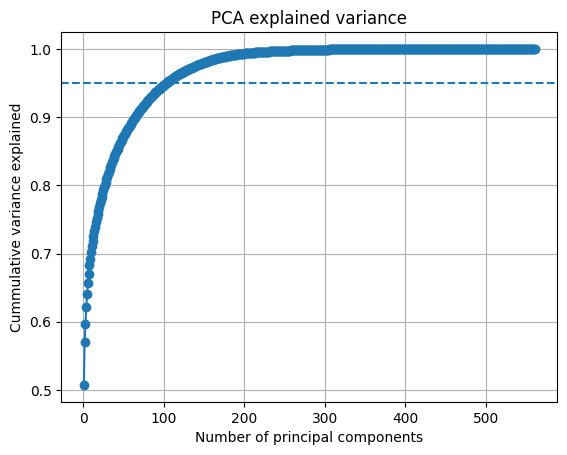
\includegraphics[width=\linewidth]{figures/fig_pca_cumvar.png}
\end{minipage}\hfill
\begin{minipage}{0.53\linewidth}
\centering
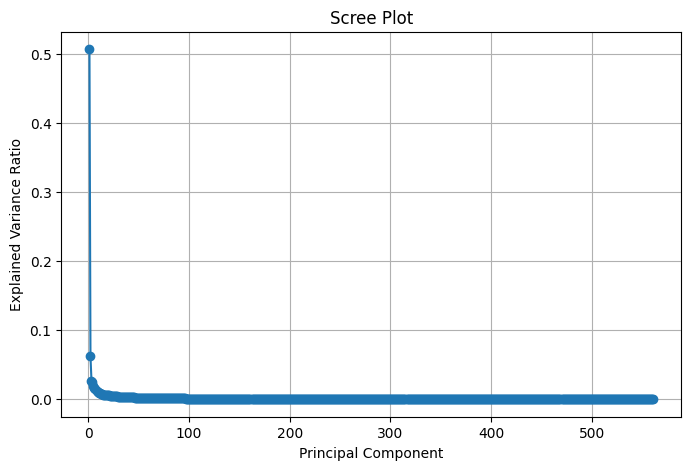
\includegraphics[width=\linewidth]{figures/fig_pca_scree.png}
\end{minipage}
\caption{Cumulative explained variance (left, dashed line = 95\%) and scree plot (right).}
\label{fig:pca}
\par\medskip
\begin{minipage}{\linewidth}
\raggedright\setlength{\parskip}{0pt}
\textbf{Inference:} The cumulative curve crosses 95\% at 104 components, so 561 correlated features can be replaced by 104 with little loss of information. The first component alone explains 50.7\% of the variance and the second 6.2\%, after which the scree curve is almost flat. The 2-D plots below therefore show only about 57\% of the variance, which means that clusters that look overlapping in 2-D may still be separable in the full space.
\end{minipage}
\end{figure}

\subsection*{K-Means: elbow and silhouette curves}
\begin{figure}[H]
\centering
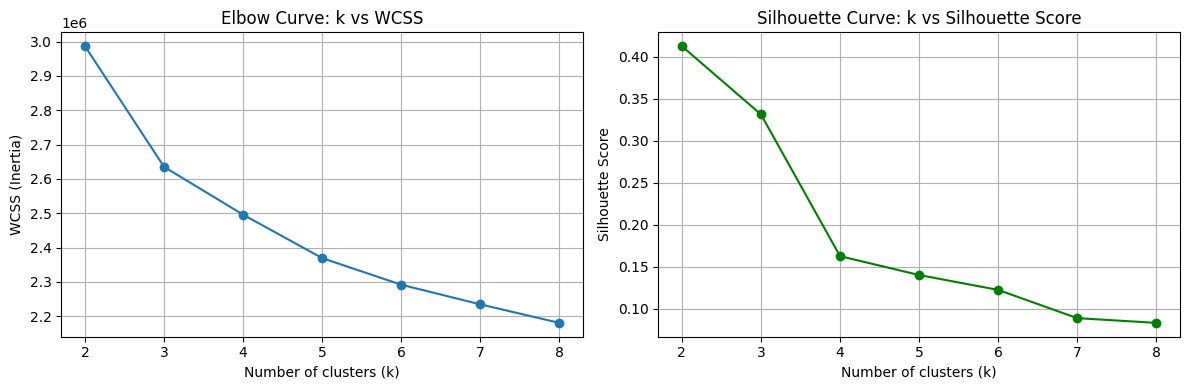
\includegraphics[width=0.95\linewidth]{figures/fig_elbow_silhouette.png}
\caption{Elbow curve ($k$ vs WCSS) and silhouette curve ($k$ vs silhouette score) for $k=2,\dots,8$.}
\label{fig:elbow}
\par\medskip
\begin{minipage}{\linewidth}
\raggedright\setlength{\parskip}{0pt}
\textbf{Inference:} WCSS falls by about 12\% from $k=2$ to $k=3$ and by 5\% or less at each following step, so the curve bends at $k=2$--3 but has no sharp elbow. The silhouette score is highest at $k=2$ (0.413) and drops quickly to 0.331 at $k=3$ and 0.162 at $k=4$. Both curves therefore point to $k=2$, the split into moving and non-moving windows. For $k>3$ the clusters are not well separated.
\end{minipage}
\end{figure}

\subsection*{DBSCAN: k-distance graph}
\begin{figure}[H]
\centering
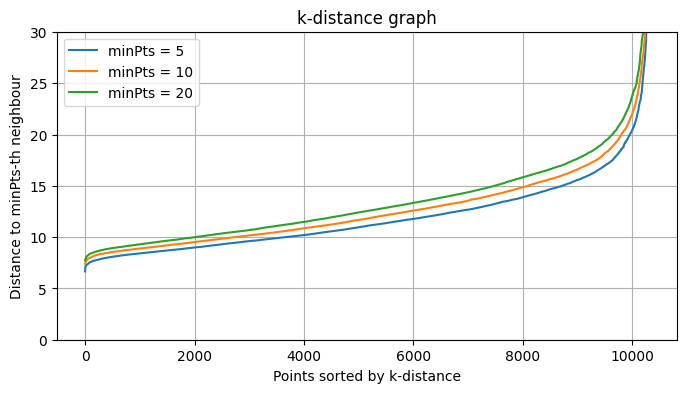
\includegraphics[width=0.6\linewidth]{figures/fig_kdistance.png}
\caption{Sorted distance of every point to its minPts-th nearest neighbour (minPts = 5, 10, 20). The vertical axis is limited to the 99th percentile.}
\label{fig:kdist}
\par\medskip
\begin{minipage}{\linewidth}
\raggedright\setlength{\parskip}{0pt}
\textbf{Inference:} For most windows the distance to the 5th--20th neighbour lies between about 7 and 20, and only the last few percent of points rise steeply. There is no single clear knee, so $\epsilon$ cannot be read from the graph alone, which is why a small grid over the percentiles was used. Values of $\epsilon$ above about 16 put more than 90\% of the points into one cluster (Section~\ref*{sec:hyper}), and the chosen $\epsilon=12.9$ lies on the lower, gently rising part of the curve.
\end{minipage}
\end{figure}

\subsection*{HAC: dendrogram}
\begin{figure}[H]
\centering
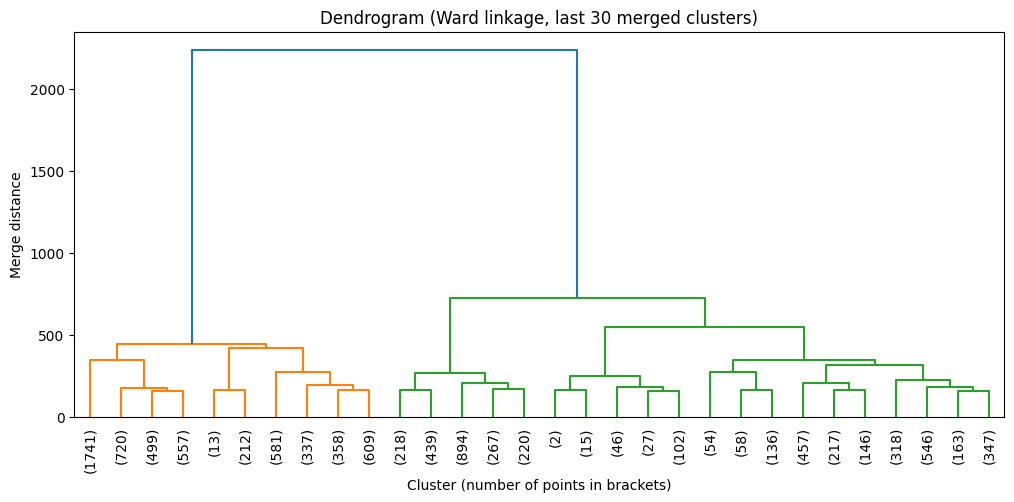
\includegraphics[width=0.72\linewidth]{figures/fig_dendrogram.png}
\caption{Dendrogram of Ward linkage (last 30 merged clusters; numbers in brackets are cluster sizes).}
\label{fig:dendro}
\par\medskip
\begin{minipage}{\linewidth}
\raggedright\setlength{\parskip}{0pt}
\textbf{Inference:} The last merge happens at a distance of about 2,200, far above all other merges (below about 750), so the data has two large branches. These are the static activities (left) and the walking activities (right). Cutting the tree just below the top gives $k=2$, and cutting lower gives $k=6$, which is the choice made in the experiment. The dendrogram agrees with the silhouette curve, which also prefers two clusters.
\end{minipage}
\end{figure}

\subsection*{Clusters in 2-D (PCA)}
\begin{figure}[H]
\centering
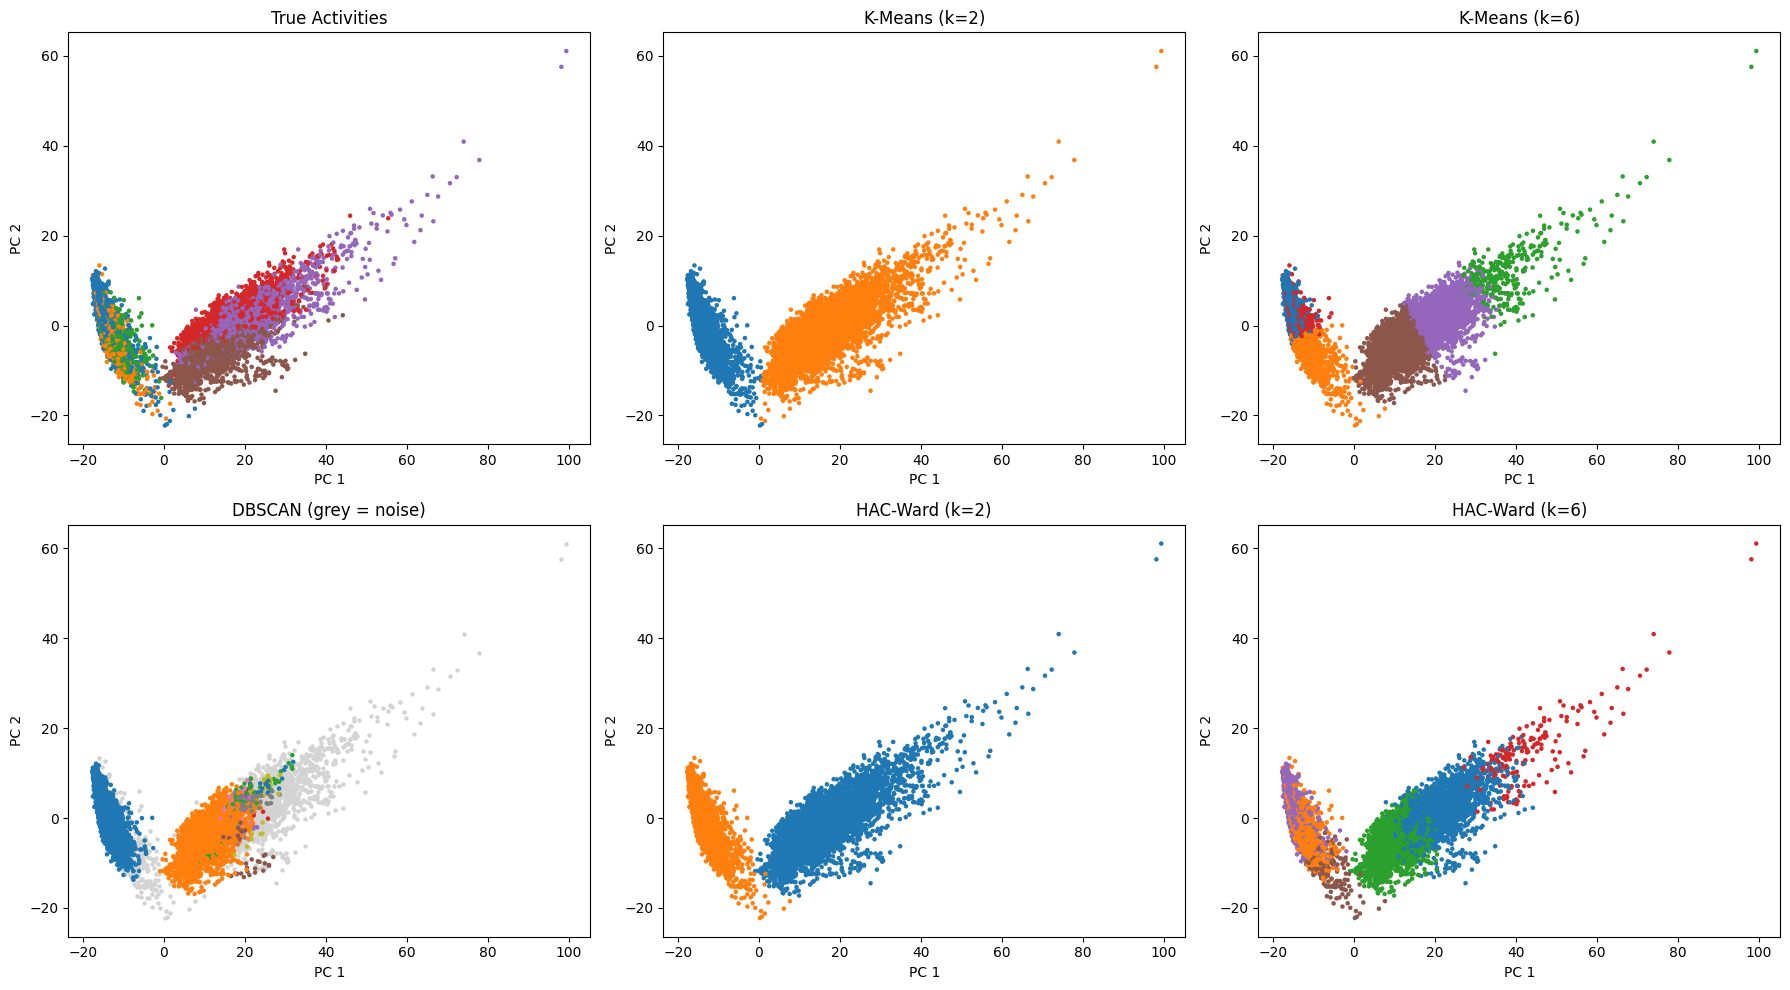
\includegraphics[width=0.95\linewidth]{figures/fig_cluster_scatter.png}
\caption{First two principal components coloured by the true activity and by each clustering result (DBSCAN noise in grey).}
\label{fig:scatter}
\par\medskip
\begin{minipage}{\linewidth}
\raggedright\setlength{\parskip}{0pt}
\textbf{Inference:} The true-activity panel shows a compact static group on the left and an elongated dynamic group on the right, and the static activities overlap each other completely. K-Means and HAC with $k=2$ reproduce these two groups almost exactly (23 wrong windows for K-Means, none for Ward). The $k=6$ solutions cut the two groups into smaller pieces, but these pieces do not match the activities. DBSCAN finds the same two dense regions and marks the sparse outer part of the dynamic group as noise.
\end{minipage}
\end{figure}

\subsection*{Confusion matrix (clusters versus activities)}
\begin{figure}[H]
\centering
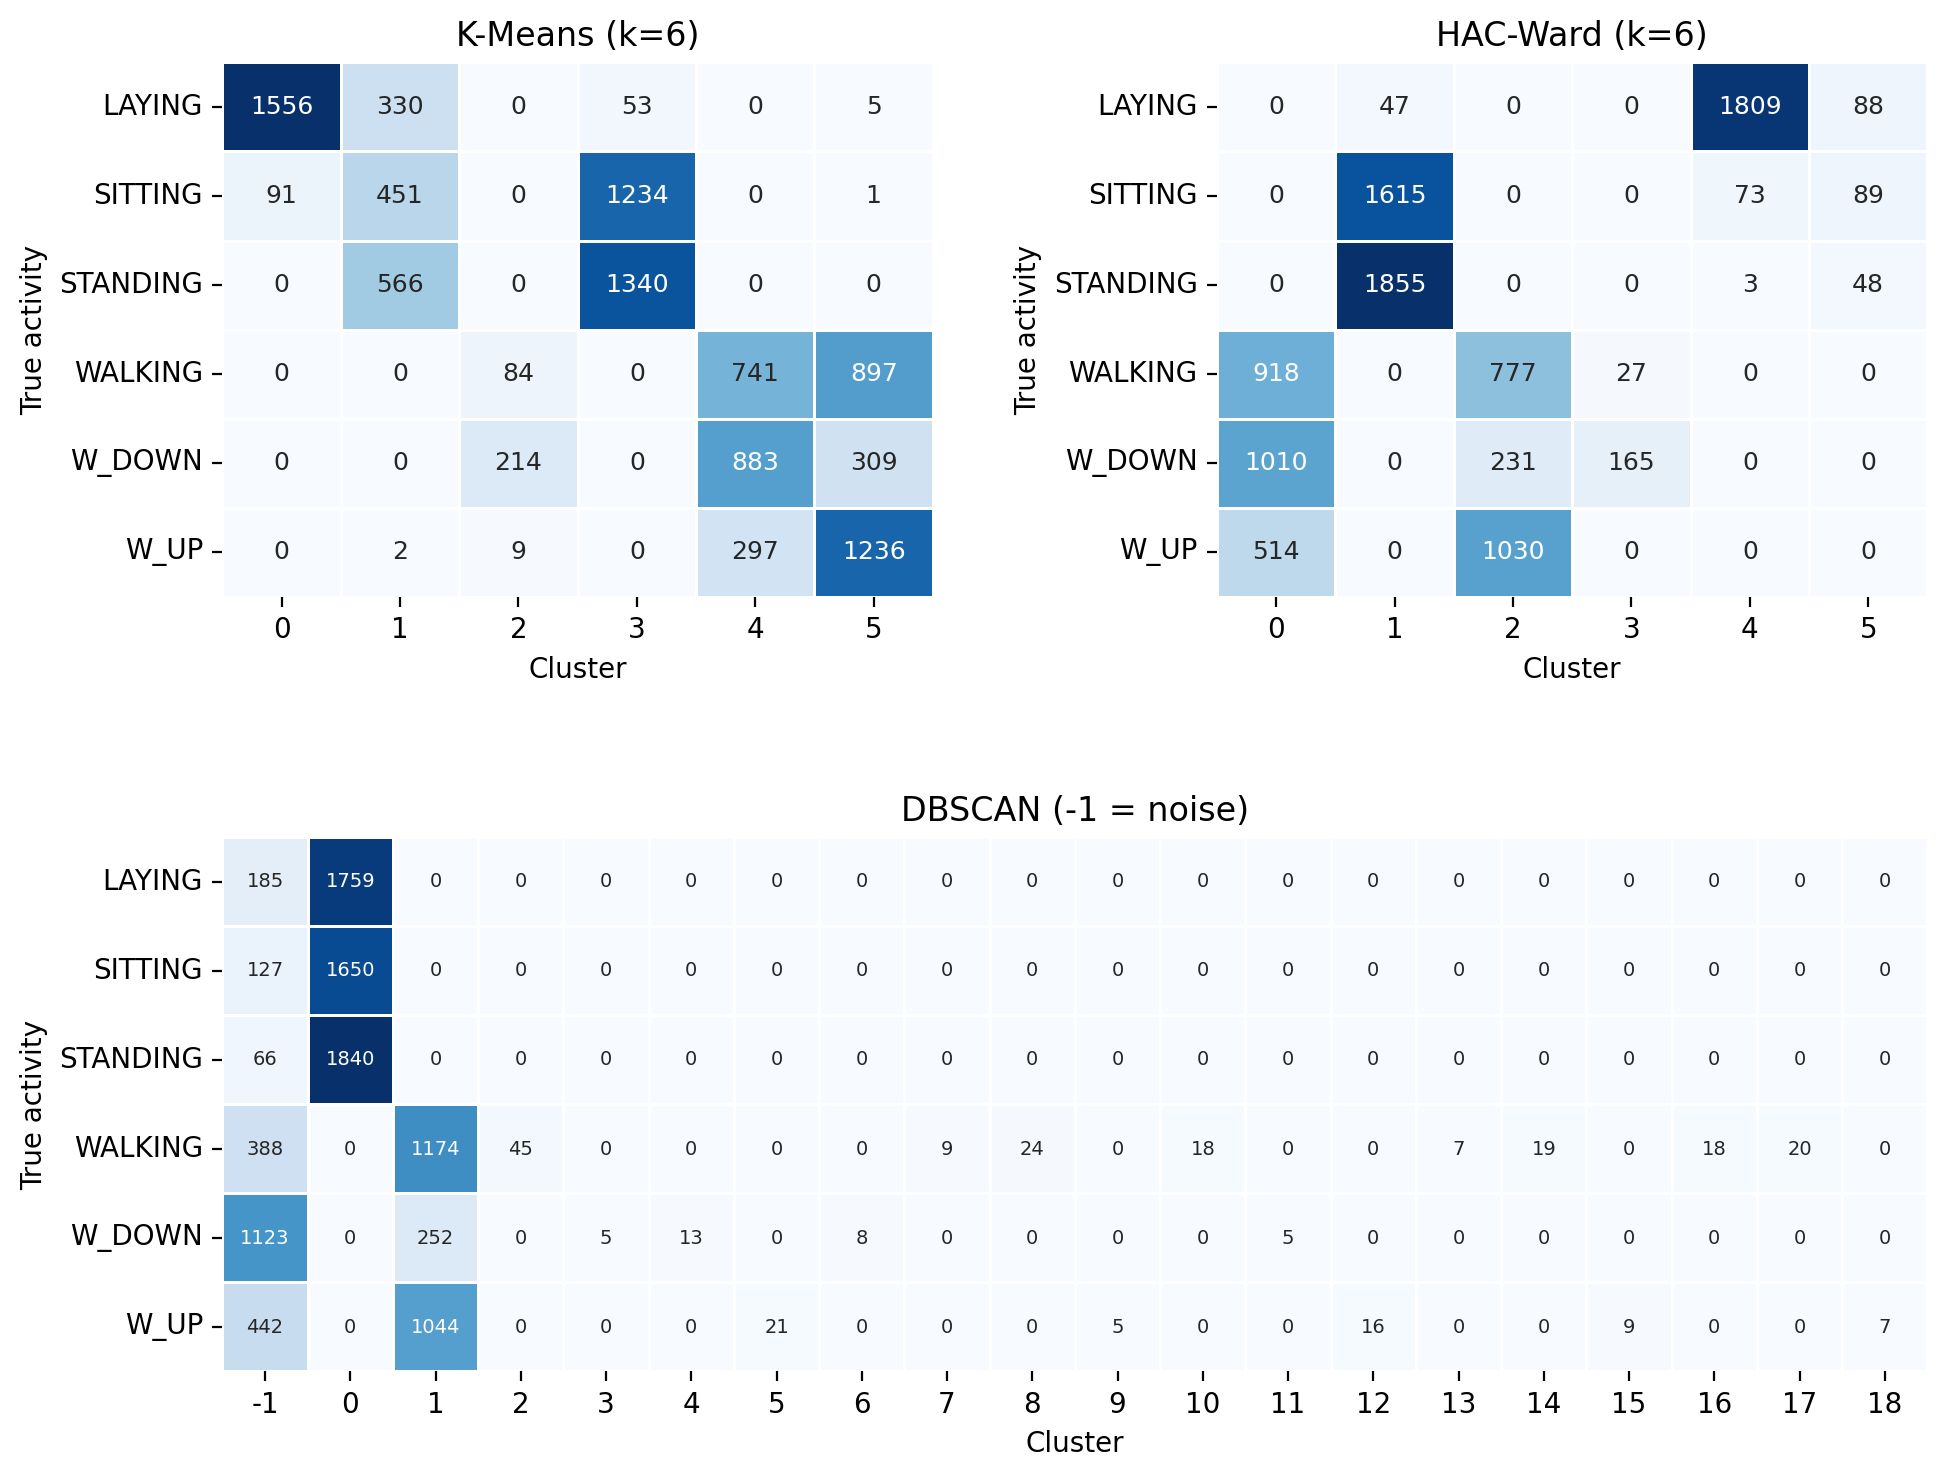
\includegraphics[width=0.8\linewidth]{figures/fig_confusion_heatmaps.png}
\caption{Number of windows of each true activity in each cluster (W\_DOWN = WALKING\_DOWNSTAIRS, W\_UP = WALKING\_UPSTAIRS).}
\label{fig:conf}
\par\medskip
\begin{minipage}{\linewidth}
\raggedright\setlength{\parskip}{0pt}
\textbf{Inference:} HAC-Ward puts 1,809 of the 1,944 LAYING windows into one cluster, but it merges SITTING and STANDING (1,615 and 1,855 windows) into another cluster. K-Means with $k=6$ splits SITTING and STANDING across two clusters in a mixed way and separates LAYING less cleanly (1,556 windows). The three walking activities are spread over three clusters by both methods. DBSCAN gives one cluster with all 5,249 static windows and marks 2,331 windows (22.6\%) as noise, of which 1,123 belong to WALKING\_DOWNSTAIRS (80\% of that activity).
\end{minipage}
\end{figure}

\subsection*{Comparison of the metrics}
\begin{figure}[H]
\centering
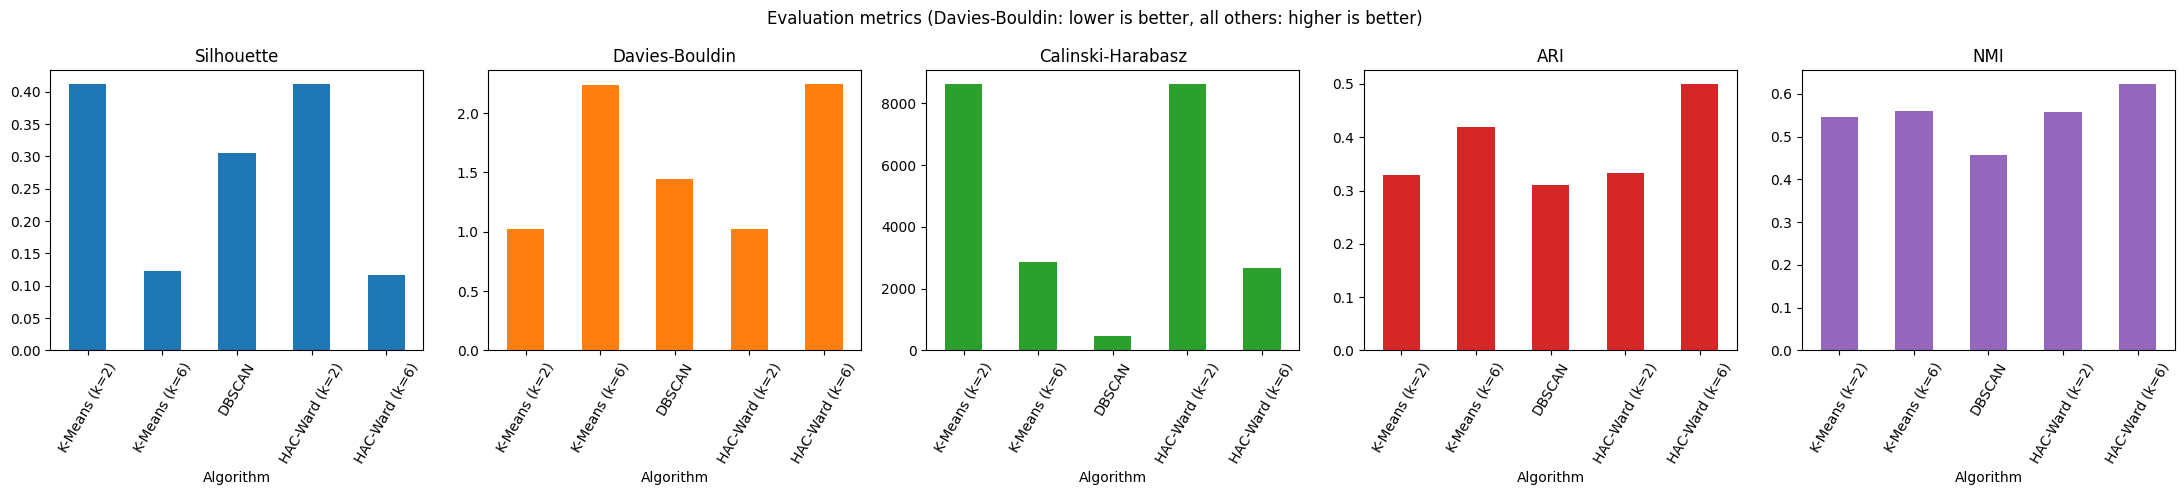
\includegraphics[width=1.0\linewidth]{figures/fig_metrics_bar.png}
\caption{Internal (silhouette, Davies--Bouldin, Calinski--Harabasz) and external (ARI, NMI) metrics of all clusterings.}
\label{fig:bars}
\par\medskip
\begin{minipage}{\linewidth}
\raggedright\setlength{\parskip}{0pt}
\textbf{Inference:} K-Means with $k=2$ is best on all three internal metrics, and HAC-Ward with $k=2$ is almost the same. HAC-Ward with $k=6$ has the best ARI (0.500) and NMI (0.624), although its internal scores are poor. DBSCAN has the lowest Calinski--Harabasz value (463) and the lowest NMI (0.456). Internal metrics reward compact and well-separated groups (moving versus not moving), while external metrics reward agreement with the six activities, so the two kinds of metrics choose different models.
\end{minipage}
\end{figure}

% ------------------------------------------------------------------
\section{Discussion}
\begin{enumerate}[leftmargin=*]
\item \textbf{Most meaningful clusters.} HAC with Ward linkage and $k=6$ agrees best with the real activities (ARI 0.500, NMI 0.624), ahead of K-Means $k=6$ (0.419, 0.559). With $k=2$, Ward separates moving from non-moving windows without a single error, and K-Means makes 23 errors out of 10,299. No method separates SITTING from STANDING.
\item \textbf{Sensitivity of K-Means to $k$.} It is strongly sensitive. The silhouette score falls from 0.413 ($k=2$) to 0.083 ($k=8$), and WCSS decreases smoothly without a sharp elbow. The internal criteria choose $k=2$, while agreement with the activities is higher for $k=6$ (ARI 0.419 against 0.330).
\item \textbf{DBSCAN, noise and small clusters.} DBSCAN detected noise (22.6\%, mostly WALKING\_DOWNSTAIRS windows, which are the most irregular) and produced 17 very small clusters (5--45 windows) in addition to two large ones. It merged the three static activities. It is also sensitive to $\epsilon$: for $\epsilon>16$ one cluster holds more than 90\% of the points (table in Section~\ref*{sec:hyper}).
\item \textbf{Effect of the linkage.} Single, complete and average linkage put 99.9\%, 95.3\% and 99.8\% of the windows into one cluster (ARI $\approx 0$), because they first separate a few outliers. Only Ward, which minimises the variance, produces balanced clusters (largest cluster 34\%).
\item \textbf{Internal metric closest to the visual impression.} The silhouette score matched the 2-D plots and the dendrogram best, as its maximum at $k=2$ agrees with the two visible groups. It must, however, be read together with the cluster sizes, because it gave single linkage the highest value (0.557) although 99.9\% of the points are in one cluster.
\end{enumerate}

\textbf{Strengths.} The full pipeline (scaling, PCA, three algorithms, five metrics) was run on all 10,299 windows, and the results are consistent across the dendrogram, the silhouette curve and the scatter plots.

\textbf{Limitations.} The 561 features are strongly correlated and the static activities overlap, so distance-based methods cannot separate sitting from standing. DBSCAN needs a single density level, which does not suit this data, and its parameters were chosen with a simple rule (the 60\% limit on the largest cluster is a choice made in this experiment). The 2-D plots show only 57\% of the variance.

\textbf{Possible improvements.} Try t-SNE or UMAP for visualisation, select or weight features (for example the gravity features that separate the static activities), try Gaussian mixture models or HDBSCAN, and normalise the features per volunteer.

% ------------------------------------------------------------------
\section{Conclusion}
K-Means, DBSCAN and Ward HAC were applied to the standardised and PCA-reduced UCI HAR data (10,299 windows, 561 features reduced to 104 components). The elbow and silhouette analysis selected $k=2$ for K-Means, and the resulting groups are moving versus not moving. HAC with Ward linkage and six clusters gave the best agreement with the six activities (ARI 0.500, NMI 0.624), whereas DBSCAN mainly detected noise and found two large clusters. Single, complete and average linkage failed because of one giant cluster. The main difficulty of the data set is the overlap of SITTING and STANDING, which none of the three algorithms could resolve.

% ------------------------------------------------------------------
\section{References}
\begingroup
\small
\renewcommand{\section}[2]{}% the heading is already printed above
\begin{thebibliography}{99}
\bibitem{anguita2013} D. Anguita, A. Ghio, L. Oneto, X. Parra, and J. L. Reyes-Ortiz, ``A public domain dataset for human activity recognition using smartphones,'' in \emph{Proc. 21st Eur. Symp. Artif. Neural Netw., Comput. Intell. Mach. Learn. (ESANN)}, Bruges, Belgium, Apr. 2013, pp. 437--442.
\bibitem{uci_har} J. Reyes-Ortiz, D. Anguita, A. Ghio, L. Oneto, and X. Parra, ``Human Activity Recognition Using Smartphones,'' UCI Machine Learning Repository, 2012. [Online]. Available: \url{https://doi.org/10.24432/C54S4K}
\bibitem{jolliffe2016} I. T. Jolliffe and J. Cadima, ``Principal component analysis: A review and recent developments,'' \emph{Phil. Trans. R. Soc. A}, vol. 374, no. 2065, Art. no. 20150202, 2016.
\bibitem{lloyd1982} S. P. Lloyd, ``Least squares quantization in PCM,'' \emph{IEEE Trans. Inf. Theory}, vol. 28, no. 2, pp. 129--137, Mar. 1982.
\bibitem{ester1996} M. Ester, H.-P. Kriegel, J. Sander, and X. Xu, ``A density-based algorithm for discovering clusters in large spatial databases with noise,'' in \emph{Proc. 2nd Int. Conf. Knowl. Discovery Data Mining (KDD)}, Portland, OR, USA, 1996, pp. 226--231.
\bibitem{ward1963} J. H. Ward, Jr., ``Hierarchical grouping to optimize an objective function,'' \emph{J. Amer. Statist. Assoc.}, vol. 58, no. 301, pp. 236--244, 1963.
\bibitem{rousseeuw1987} P. J. Rousseeuw, ``Silhouettes: A graphical aid to the interpretation and validation of cluster analysis,'' \emph{J. Comput. Appl. Math.}, vol. 20, pp. 53--65, 1987.
\bibitem{davies1979} D. L. Davies and D. W. Bouldin, ``A cluster separation measure,'' \emph{IEEE Trans. Pattern Anal. Mach. Intell.}, vol. PAMI-1, no. 2, pp. 224--227, Apr. 1979.
\bibitem{calinski1974} T. Cali\'{n}ski and J. Harabasz, ``A dendrite method for cluster analysis,'' \emph{Commun. Statist.}, vol. 3, no. 1, pp. 1--27, 1974.
\bibitem{hubert1985} L. Hubert and P. Arabie, ``Comparing partitions,'' \emph{J. Classification}, vol. 2, no. 1, pp. 193--218, 1985.
\bibitem{strehl2002} A. Strehl and J. Ghosh, ``Cluster ensembles---A knowledge reuse framework for combining multiple partitions,'' \emph{J. Mach. Learn. Res.}, vol. 3, pp. 583--617, 2002.
\bibitem{pedregosa2011} F. Pedregosa \emph{et al.}, ``Scikit-learn: Machine learning in Python,'' \emph{J. Mach. Learn. Res.}, vol. 12, pp. 2825--2830, 2011.
\end{thebibliography}
\endgroup

\end{document}
